% label prefix for this part: dat
\part{Project dat}\label{part:dat}

\chapter{Einführung}

In der heutigen Gesellschaft wird der Austausch von Daten immer wichtiger. Vermehrt werden grosse Datenmengen unterschiedlichster Art - aus Forschung, Regierung oder zivilen Kreisen - zur allgemeinen Verwendung angeboten. Nicht nur die Art der Daten ist jedoch vielfältig, sondern auch Datenformat oder Zugriffsart unterscheiden sich.

Das \gls{dat}-Projekt hat das Ziel, die Integration sowie einen einheitlichen Zugriff solcher Datenquellen vereinfachen.

Als erstes Ziel dieser Arbeit sollte das noch junge Projekt \gls{dat} anlysiert und dessen genaue Funktionalität und Funktionsweise dokumentiert werden. Aufgrund der Tatsache, dass \gls{dat} noch relativ neu ist und sich in der Alphaphase befindet, ist das Projekt nur wenig und sehr verstreut dokumentiert. \Gls{dat} hat im Jahr 2014 einen Gesamtbetrag von \SI{310000}[\$]{} von der \gls{knight-foundation} sowie der \gls{sloan-foundation} zur Weiterentwicklung des Projekts erhalten, was als Indiz für ein vielversprechendes Projekt gilt.

\section{Was ist dat?} % https://github.com/maxogden/dat/blob/master/docs/what-is-dat.md

Das dat-Projekt hat folgende Ziele\cite{what-is-dat}: 

\begin{itemize}
\item Daten sollen automatisch zwischen unterschiedlichen dat-Instanzen synchronisiert werden können. 
\item Unterstützung grosser Datenmengen\footnote{Milliarden von Datensätzen bzw. Speicherbedarf im \si{\tera\byte}-Bereich}, evtl. mit häufigen Aktualisierungen
\item Unterstützung von Daten in Tabellenform oder unstrukturiert
\item Plugin-basierte Schnittstelle zu bestehenden Datenbanken/Formaten
\item Unterstützung für automatisierte Workflows
\end{itemize}

% https://github.com/maxogden/dat/blob/master/docs/js-api.md#transformations
Für den Umgang mit verschiedenen Datenformaten können Transformationen\cite[transformations]{dat-js-api} definiert werden, welche entweder vor Schreib- oder nach Lese-Operationen ausgeführt werden.


\section{CLI}

%https://github.com/maxogden/dat/blob/master/docs/cli-usage.md

Das \gls{dat} \gls{cli} ``\texttt{dat}'' ist das einzige Werkzeug um ohne API mit dem Repository zu interagieren und bietet folgende Basisfunktionalität:

\begin{itemize}
  \item Erstellung neuer dat Repositories/Intanzen mit \mintinline{console}{$ dat init}
  \item Import von CSV oder JSON Dateien mit \mintinline{console}{$ dat import}
  \item \gls{dat} Server und Webfrontend starten mit \mintinline{console}{$ dat listen}
  \item Klonen eines kompletten\footnote{Samt aller Historie} remote Repositories \gls{dat} Repostitories analog Git mit \mintinline{console}{$ dat clone}
  \item Lokale Änderungen ebenfalls analog Git wieder zurück ins remote Repository synchronisieren mit \mintinline{console}{$ dat push}
  \item Rudimentäre Manipulation und Ausgabe von einzelnen Zeilen des Repositories mit \mintinline{console}{$ dat rows} bzw. \mintinline{console}{$ dat cat}
\end{itemize}

Die abschliessende Liste von zurzeit unterstützten Befehlen ist in 
\vref{app:dat-help} zu finden. Für fortgeschrittenere Verwendung ist das \gls{cli} jedoch nicht geeignet, da viele Optionen fehlen. Stattdessen sollte das JavaScript-API verwendet werden.

Spätere Versionen sollen auch Branches erlauben sowie mit Änderungskonflikten umgehen können.

\section{Frontend}

\Gls{dat} bietet ein minimales Webfrontend welches ähnliche Operationen wie mit dem \gls{cli} wie z.B. Import/Export sowie betrachten der Datensätze ermöglicht. Einen Ausschnitt ist folgender \cref{fig:dat:webfrontend} zu sehen.

\begin{figure}[H]
  \centering
  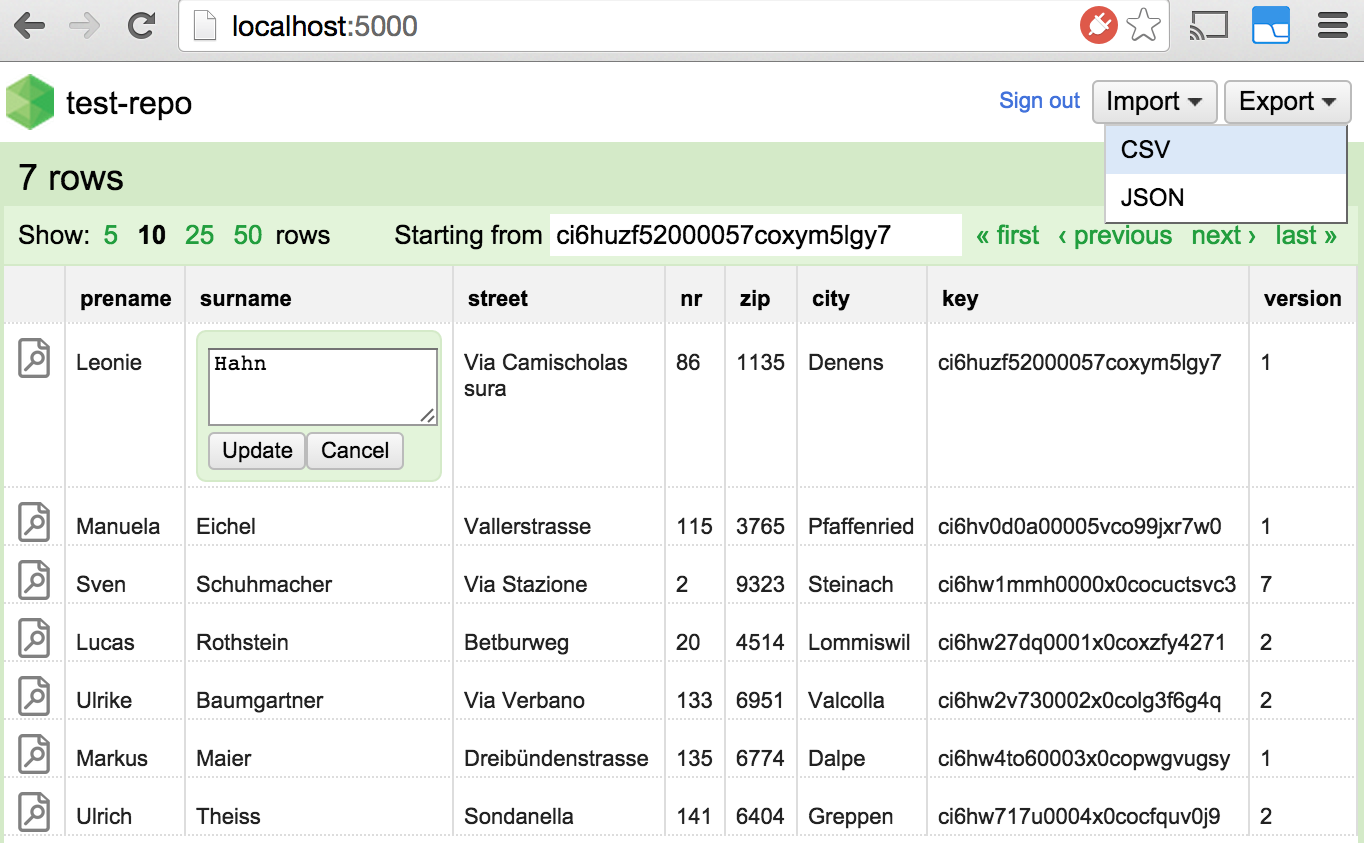
\includegraphics[width=0.8\textwidth]{fig/webfrontend}
  \caption{dat Webfrontend}
  \label{fig:dat:webfrontend}
\end{figure}


\section{Architektur}
% diagramm, requirements, interfaces, ...

% http://dat-data.com/docs.html: "Q:If I have multiple different tables that I want to store, would I create a separate dat repo for each? Can a single dat repo store multiple tables? A: Each dat repo is only one table."

dat speichert Daten auf zwei verschiedene Arten:
\begin{itemize}
\item Für Tabellen-Daten wird LevelDB verwendet. Da LevelDB ein austauschbares Backend hat können diese Daten auch in einer SQL-Datenbank wie Postgres gespeichert werden.
\item Blob-Daten werden standardmässig im File-System per local-blob-store gespeichert. Dies kann ebenfalls durch eine kompatible Implementation ausgetauscht werden.
\end{itemize}

\begin{figure}[H]
  \centering
  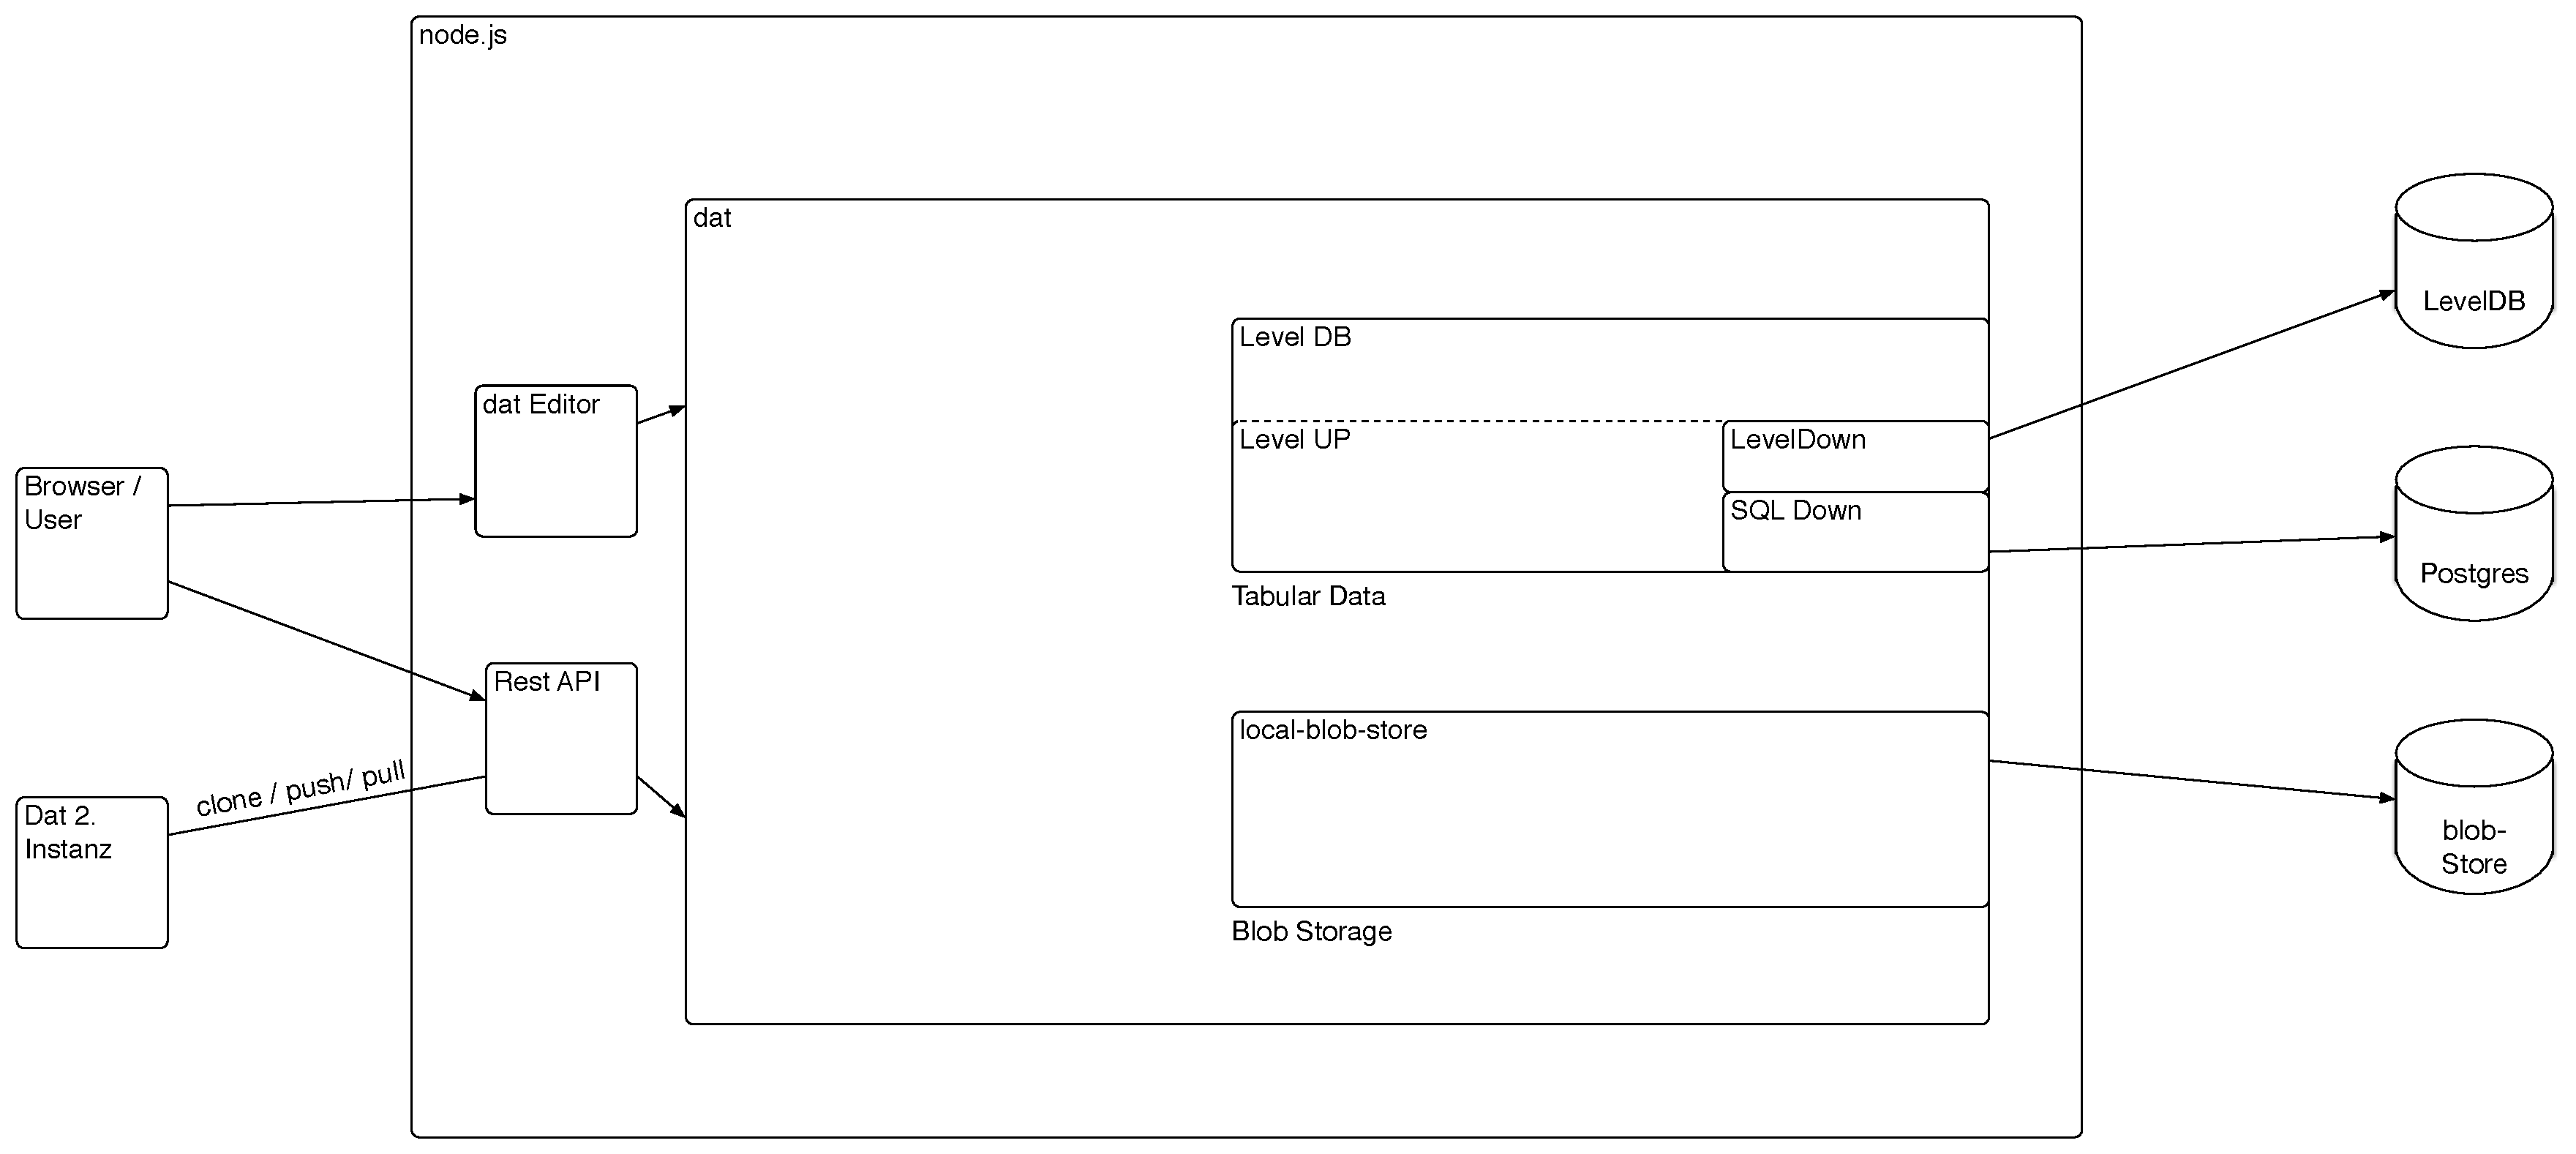
\includegraphics[width=\linewidth,clip]{fig/dat-architecture}
  \caption{dat Architektur-Übersicht}
  \label{fig:dat-architecture-overview}
\end{figure}

Direkt mit dat wird auch der dat-editor geliefert, welcher als rudimentäres Web-GUI dient. Der Editor sowie das REST-API werden gestartet, wenn \mintinline{console}{dat listen} aufgerufen wird. Andere dat-Instanzen verwenden das REST-API für die Synchronisation.

\begin{figure}[H]
  \centering
  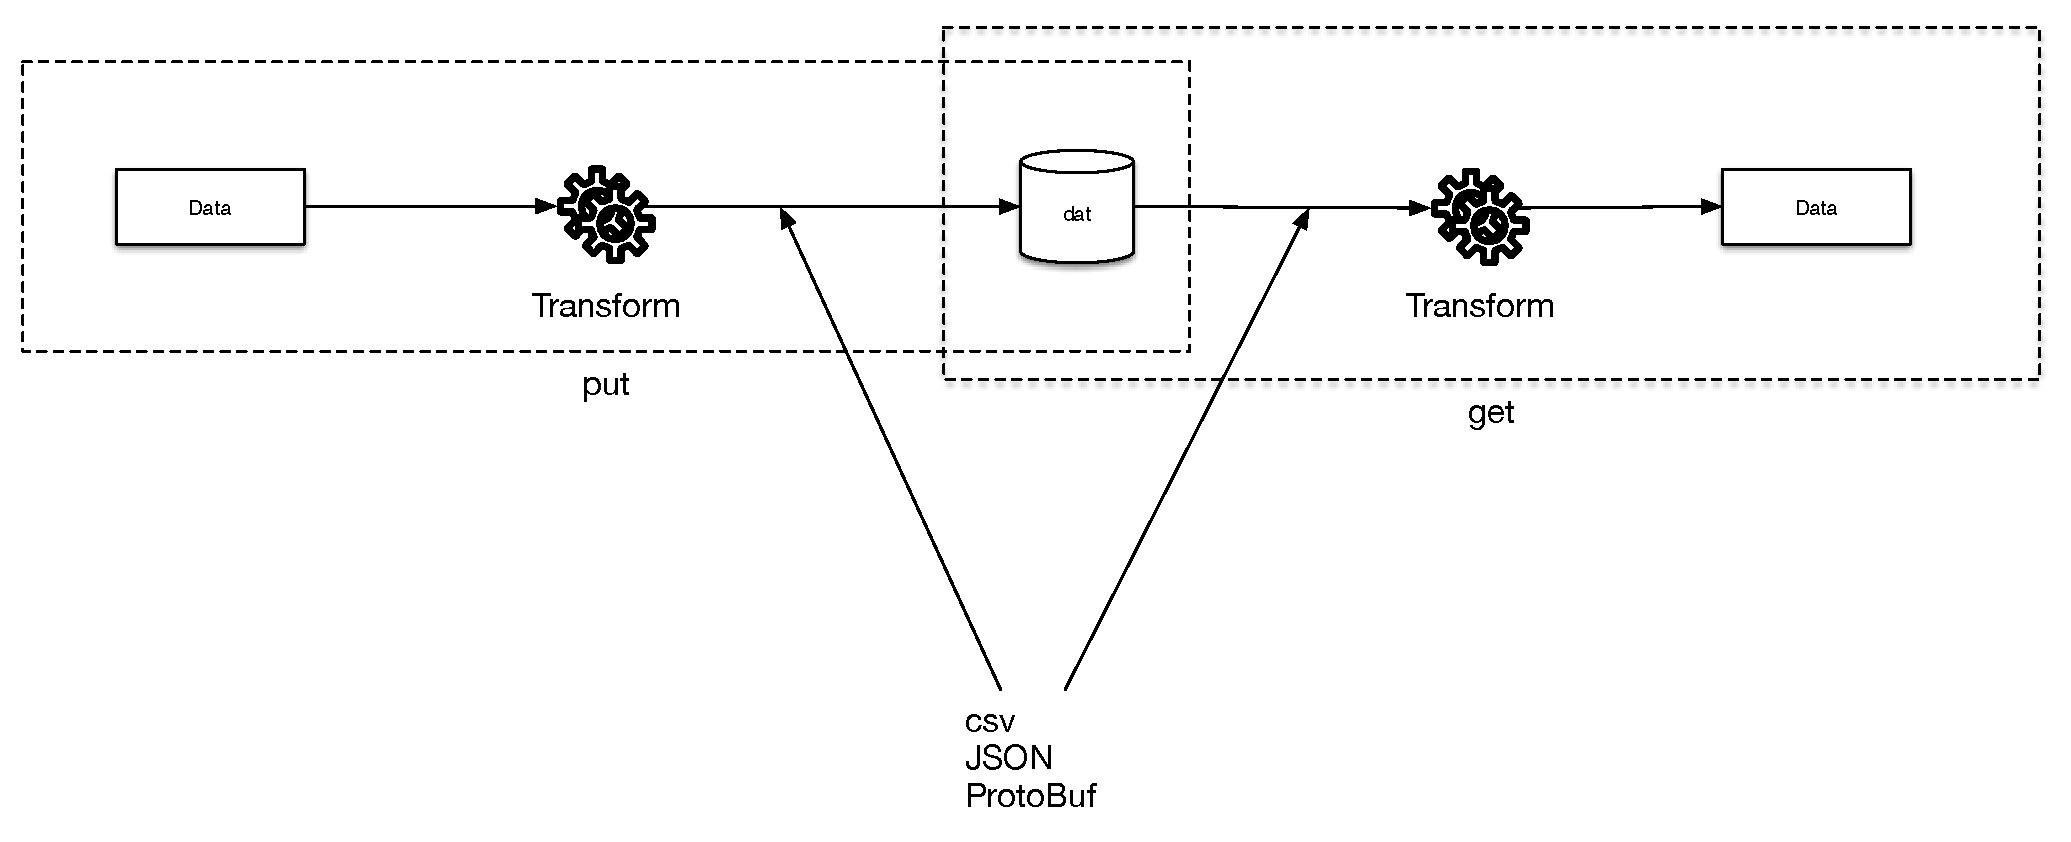
\includegraphics[width=\linewidth,clip]{fig/dat-pipeline}
  \caption{dat Daten-Pipelines}
  \label{fig:dat-architecture-pipeline}
\end{figure}

Mithilfe des Sub-Projekts \texttt{gasket} können sogenannte Daten-Pipelines definiert werden. Diese dienen dazu, Daten abzurufen, zu transformieren und schliesslich in dat zu speichern, bzw. Daten aus dat zu lesen, zu transformieren und schliesslich abzuliefern.

\section{Use Cases}
In diesem Abschnitt werden mögliche Verwendungszwecke von \gls{dat} aufgezeigt.

\subsection{Astronomie \textendash\ Trillian} 
% https://github.com/maxogden/dat/issues/172
% https://github.com/trillian/trillian
% http://trillianverse.com (nicht verfügbar 2015-02-23)
In der Astronomie fallen riesige Datenmengen an. Teilweise werden diese als grosse Daten-Releases zur Verfügung gestellt (z.B. Sloan Digital Sky Survey), welche frühere Releases komplett ersetzen. Andere Projekte stellen inkrementelle Updates zur Verfügung (z.B. Hubble). Viele Astronomie-Institute haben weder die Mittel noch das Know-how, mit solchen Datenmengen umgehen zu können. Das Trillian-Projekt kümmert sich um die Verwaltung dieser Daten und bietet eine Compute-Engine an, um neue Modelle anhand der vorhandenen Daten zu testen.

dat soll für den Import und die Indexierung der Daten verwendet werden.

Siehe auch \url{https://github.com/maxogden/dat/issues/172}.

\subsection{Regierung \textendash\ Sammlung von Daten} % https://github.com/maxogden/dat/issues/153
Für Statistik- oder Regulierungszwecke sammeln Regierungen Daten von unterschiedlichsten Betrieben. Diese Daten müssen oft über ein mehr oder weniger brauchbares Portal abgeliefert werden.

Die Verwendung von dat bringt folgende Vorteile:
\begin{itemize}
\item Ermöglicht die Prüfung von Daten beim Import, bereits vor der Ablieferung der Daten
\item Ermöglicht Ergänzung oder Korrektur von bereits abgelieferten Daten.
\item Ersatz der bisher verwendeten, für jede Regierungsstelle neu kreierten und teuren, Portale durch eine standardisierte Lösung.
\end{itemize}

Siehe auch \url{https://github.com/maxogden/dat/issues/153}.

\chapter{Erweiterung}

Dieses Kapitel beschreibt die Möglichkeiten wie \gls{dat} mittels Schnittstellen und Konfiguration über dessen Basisfunktionalität eines simplen tabellen-artigen Speichers hinaus verwendet werden kann.

\section{Datscript} %https://github.com/datproject/datscript

Datscript ist eine für spezielle \gls{dsl} für \gls{dat} die es ermöglicht Befehle zu konfigurieren sowie mehrere Befehle zu sogenannten Pipelines zu verknüpfen. Obschon Datscript an diversen Stellen erwähnt wird und ein Repository auf GitHub\footnote{Lediglich ein Beispiel für das Konzept, keinerlei Programmcode vorhanden} besteht, so ist es bisher lediglich ein Konzept und wurde noch nicht implementiert. Es ist zu vermuten, das Datscript gar nicht implementiert wird und durch das in \cref{sec:dat:gasket} beschriebene Gasket ersetzt wurde.


\begin{srclst}{bash}{Datscript Beispiel}
# validate cli args
args [url]

# import another datscript file
import foo.ds

# set env var for all run commands to use
env foo = "bar"

# run a pipeline (hoists)
run pipeline import

# run a command (from node_modules/.bin or PATH)
run foobar

# define main (default) pipeline
pipeline main
  run pipeline import

# define pipeline w/ piping
pipeline import
  run foobar | run dat import --json
\end{srclst}

\section{Gasket}\label{sec:dat:gasket} % https://github.com/datproject/gasket
Gasket ist eine Node.js-basierte Pipeline-Engine. Die Konfiguration geschieht entweder im JSON-Format direkt in \path{package.json}, oder aber in einem Node.js-Modul. Unterstützt wird die Ausführung von externen Programmen, oder die Verwendung von Node.js-Modulen.

Ein Beispiel einer trivialen \path{package.json} Konfiguration wird in \cref{lst:dat:gasket-example} aufgezeigt und gibt lediglich ``HELLO WORLD'' aus .

\begin{srclst}[label=lst:dat:gasket-example]{json}{Offizielles Gasket Beispiel}
{
  "name": "my-test-app",
  "dependencies" : {
    "transform-uppercase": "^1.0.0"
  },
  "gasket": {
    "example": [
      {
        "command": "echo hello world",
        "type": "pipe"
      },
      {
        "command": "transform-uppercase",
        "type": "pipe"
      }
    ]
  }
}
\end{srclst}


\section{Schnittstellen / API}

\subsection{REST}
% https://github.com/maxogden/dat/blob/master/docs/rest-api.md

Der dat-Server kann von jeder dat-Instanz durch \mintinline{console}{$ dat listen} gestartet werden.

dat implementiert aktuell nur HTTP Basic Authentication mit einem einzelnen Benutzer, welcher in dat.json konfiguriert werden kann. 

Falls ein Admin-Benutzer konfiguriert ist, können nur angemeldete Sessions Daten ändern, es können jedoch immer noch alle Daten von allen Benutzern gelesen werden.
% https://github.com/maxogden/dat/blob/master/docs/dat-json-config.md#adminuser-adminpass

SSL wird bisher nicht unterstützt.

\paragraph{GET /} ~\\
Liefert die Webapplikation dat-editor aus.

\paragraph{Antwort GET /api} ~\\
Liefert allgemeine Informationen zur dat-Instanz
\begin{srclst}{json}{GET /api}
    {
        "dat":"Hello",
        "version":"6.9.6",
        "changes":2,
        "name":"dat-test",
        "rows":53,
        "approximateSize":{
            "rows":"3 kB"
        }
    }
\end{srclst}

\paragraph{GET /api/rows} ~\\
Liefert eine Liste von Einträgen (Default: 50 Einträge).
% http://www.fakenamegenerator.com/gen-random-gr-sz.php ftw
\begin{srclst}{json}{Antwort GET /api/rows}
{
    "rows": [
        {
            "prename":"Leonie", "surname":"Hahn", 
            "street":"Via Camischolas sura", "nr":"86", 
            "zip":"1135", "city":"Denens", 
            "key":"ci6huzf52000057coxym5lgy7", "version":1
        },
        {
            "prename":"Manuela", "surname":"Eichel", 
            "street":"Vallerstrasse", "nr":"115",
            "zip":"3765", "city":"Pfaffenried", 
            "key":"ci6hv0d0a00005vco99jxr7w0", "version":1
        },
        ...
    ]
}
\end{srclst}

\paragraph{GET /api/rows/:key} ~\\
Liefert den Eintrag mit dem angegebenen Schlüssel, oder eine Fehlermeldung.

\begin{srclst}{json}{Antwort GET /api/rows/ci6huzf52000057coxym5lgy7}
{
    "prename":"Leonie", "surname":"Hahn", 
    "street":"Via Camischolas sura", "nr":"86", 
    "zip":"1135", "city":"Denens", 
    "key":"ci6huzf52000057coxym5lgy7", "version":1
}
\end{srclst}

\paragraph{POST /api/rows} ~\\
Fügt einen neuen Datensatz hinzu. Die Daten müssen als JSON vorliegen.

Die Antwort besteht entweder aus einer Konflikt-Meldung, oder aus dem neu hinzu gefügten Datensatz.

\begin{srclst}{console}{POST /api/rows}
$ curl -H 'Content-Type: application/json' -d '{"prename":"Markus", "surname":"Maier", "street":"Dreibündenstrasse", "nr":"135", "zip":"6774", "city":"Dalpe"}' -X POST localhost:6461/api/rows
{"prename":"Markus", "surname":"Maier", "street":"Dreibündenstrasse", "nr":"135", "zip":"6774", "city":"Dalpe", "key":"ci6hw717u0004x0cocfquv0j9", "version":1}
\end{srclst}

\paragraph{GET /api/rows/:key/:filename} ~\\
Liefert das Blob mit dem entsprechenden Filenamen, oder eine Fehlermeldung falls nicht verfügbar.

\paragraph{POST /api/rows/:key/:filename} ~\\
Fügt ein neues Blob zum angegebenen Datensatz hinzu. Der Datensatz muss bereits existieren, und die aktuelle Version des Datensatzes muss im Query-String angegeben werden: \\
\mintinline{http}{POST /api/rows/foo/photo.jpg?version=1 HTTP/1.1}

\paragraph{GET /api/session} ~\\
Liefert Informationen zur aktuellen Session. Dieser Aufruf kann auch zur Anmeldung per Basic Authentication verwendet werden.

\paragraph{GET /api/login} ~\\
Selbe Funktionalität wie /api/session, setzt jedoch den HTTP-Header ``Basic realm="Secure Area"'', so dass Browser ein Login-Fenster anzeigen.

\paragraph{GET /api/logout} ~\\
Zerstört die aktuelle Session und entfernt Client-Side Cookies.

\paragraph{GET /api/changes} ~\\
Liefert eine Json-formatierte Version des Change Streams (siehe auch JavaScript-API createChangesStream).

\paragraph{GET /api/csv} ~\\
Liefert eine CSV-Datei mit der letzten Version der Daten.

\paragraph{POST /api/bulk} ~\\
Ermöglicht das Einfügen von mehreren Datensätzen gleichzeitig. Unterstützt werden JSON (Content-Type \texttt{application/json}) und CSV (Content-Type \texttt{text/csv}).

Falls die Daten akzeptiert werden besteht die Antwort aus einer Liste von JSON-Objekten mit Key und Version für die neu eingefügten Datensätze, andernfalls aus einem HTTP-Fehler.

\begin{srclst}{json}{GET /api/metadata}
{
    "changes":15, 
    "liveBackup":false, 
    "columns":["prename","surname","street","nr","zip","city","version:"]
}
\end{srclst}

\paragraph{GET /api/manifest} ~\\
Liefert ein JSON-Objekt mit Informationen zum DB-Backend. Dies wird für RPC verwendet (siehe \path{/api/rpc}).

\paragraph{POST /api/rpc} ~\\
Ein Server-Endpunkt für multilevel (Node.js-Modul).

\paragraph{GET /api/metadata} ~\\
Liefert Informationen zum Schema. Diese Daten werden während der Replikation verwendet.

\paragraph{GET /api/replicator/receive und GET /api/replicator/send} ~\\
Wird für Replikation verwendet.

\subsection{JavaScript}
%https://github.com/maxogden/dat/blob/master/docs/js-api.md
dat kommt als Node.js-Modul daher und ist die einzige Möglichkeit überhaupt um auf performante Art und Weise das \gls{dat} Repository zu manipulieren. Das \gls{cli} verwendet intern ebenfalls die JavaScript API. Dieser Abschnitt zeigt auf welche Interaktionsmöglichkeit mit dem Repository via JavaScript API möglich ist.

\begin{srclst}{js}{Laden des dat-Moduls}
var dat = require('dat')
\end{srclst}

\paragraph{\texttt{var db = \parahighlight{dat}([path], [options], [onReady])}} ~\\

Erstellt eine neue oder öffnet eine bereits bestehende dat-Datenbank. Alle Parameter sind optional.

\begin{description}
\item[path (string)] Pfad zum Verzeichnis, welches das \texttt{.dat}-Verzeichnis enthält. Falls kein \texttt{.dat}-Verzeichnis existiert wird ein neues erstellt. Default ist \mintinline{js}{process.cwd()}.
\item[options (object)] Weitere Konfigurations-Parameter:
    \begin{description}
    \item[init] Wenn \mintinline{js}{false} erstellt dat keine neue Datenbank beim Initialisieren. Default: \mintinline{js}{true}.
    \item[storage] Wenn \mintinline{js}{false} versucht dat nicht beim Initialisieren die Datenbank zu lesen. Default: \mintinline{js}{true}.
    \item[path] Alternative zum Konstruktor-Argument.
    \item[adminUser, adminPass] Wird als Benutzer/Passwort verwendet für HTTP Basic Authentication wenn beide konfiguriert sind.
    \item[leveldown] Benutzerdefiniertes \texttt{leveldown}-Backend. Default: \mintinline{js}{require('leveldown-prebuilt')}
    \item[db] Benutzerdefinierte \texttt{levelup}-Instanz. Wenn diese Option vorhanden ist wird die \texttt{leveldown}-Option ignoriert und alle Tabellen-basierte Daten werden in dieser DB-Instanz gespeichert.
    \item[blobs] Benutzerdefinierte \texttt{blob}-Datenbank. Default: \mintinline{js}{require('lib/blobs.js')}
    \item[replicator] Benutzerdefinierte Replicator-Instanz. Default: \mintinline{js}{require('lib/replicator.js')}
    \item[remoteAddress] Falls angegeben started dat im RPC Client-Modus. Default: \mintinline{js}{undefined}
    \item[manifest] Wenn \texttt{remoteAddress} gesetzt ist wird dies als Manifest für RPC verwendet.
    \item[skim] Wenn \mintinline{js}{true} wird lazy auf Blobs von einer nicht-lokalen Quelle zugegriffen. Default: \mintinline{js}{false}.
    \item[transformations] siehe Transformationen
    \item[hooks] siehe Transformationen
    \end{description}
\item[onReady: (err)] Wird aufgerufen nachdem dat initialisiert wurde. Wenn \texttt{err} gesetzt ist trat ein Fehler auf.
\end{description}
 
\subparagraph{Transformationen}
Transformationen können vor \texttt{put}- oder nach \texttt{get}-Operationen ausgeführt werden. Die Konfiguration erfolgt über den \texttt{options}-Parameter im Konstruktor.

\begin{srclst}{js}{Beispiel einer Transformations-Konfiguration}
{
  "transformations": {
    "get": "transform-uppercase",
    "put": [{"module": "./lowercase-stream.js"}]
  }
}
\end{srclst}

Folgende Datentypen sind möglich:
\begin{description}
\item[string] Ausführbarer Befehl, um die Daten zu transformieren. Der Befehl erhält durch Zeilenumbrüche getrennte JSON-Datensätze (\acs{ndjson}) in \texttt{STDIN}. Nach der Transformation werden die Daten wieder als JSON auf \texttt{STDOUT} erwartet.
\item[object] Objekt mit einem der folgenden Feldern:
    \begin{description}
    \item[command] Gleiche Funktionalität wie oben
    \item[module] Per \texttt{require()} ladbares Node.js-Modul. Das Modul muss einen Streams2-Passthrough Stream exportieren mit \mintinline{js}{objectMode: true}. Falls das Modul installiert werden muss, sollte die Abhängigkeit direkt in package.json eingetragen werden.
    \end{description}
\item[array] Array von Transformationen, welche nacheinander ausgeführt werden.
\end{description}

\subparagraph{Hooks}
Aktuell existiert nur ein einzelner Hook:
\begin{description}
\item[listen] Wird ausgeführt, wenn der dat-Server an einen Port bindet.
\end{description}

Ein Hook muss als Node.js-Modul, wie in \cref{lst:dat:hook} gezeigt, vorliegen.

\begin{srclst}[label=lst:dat:hook]{js}{Hook-Beispiel}
module.exports = function hook(dat, done) {
  // do stuff with dat

  // must call done when the hook is done initializing, even if you call it immediately
  done()
}
\end{srclst}

Nach erfolgreicher Initialisierung muss die Funktion \texttt{done} zwingend aufgerufen werden!

% get

\paragraph{\texttt{\parahighlight{get}(key, [options], callback: (error, value))}} ~\\
Findet den zum Key gehörenden Datensatz, falls vorhanden, und übergibt das Resultat an den callback.
\begin{description}
\item[options] Objekt mit folgenden Feldern:
\begin{description}
\item[version] Erlaubt das finden einer spezifischen Version. Default: aktuellste Version.
\end{description}
\end{description}
% put 

\paragraph{\texttt{\parahighlight{put}([key], value, [options], callback: (error, newVersion))}} ~\\
Fügt einen neuen Datensatz in die Datenbank ein. Der Key kann optional als Parameter oder als \texttt{value.key} übergeben werden.

Bereits bestehende Einträge werden nur überschrieben, wenn \texttt{value.version} mit der aktuellsten in der Datenbank existierenden Version übereinstimmt. Andernfalls tritt ein Konflikt-Fehler auf.

\begin{description}
\item[options] Objekt mit folgenden Feldern:
    \begin{description}
    \item[force] Wenn \mintinline{js}{true} wird der Versions-Check übersprungen und Konflikte ignoriert. Für die neuen Daten wird eine neue Version erzeugt.
    \end{description}
\end{description}

% delete

\paragraph{\texttt{\parahighlight{delete}(key, callback: (error, newVersion))}} ~\\
Markiert den Key als gelöscht. Achtung: Alte Versionen bleiben erhalten und können weiterhin abgerufen werden.

% createReadStream

\paragraph{\texttt{var readStream = db.\parahighlight{createReadStream}([options])}} ~\\
Liefert einen lesbaren Stream der neusten Versionen aller Datensätze.

Die Einträge werden als \mintinline{js}{ {key: key, value: value} } geliefert.

\begin{description}
\item[options] Objekt mit folgenden Feldern:
    \begin{description}
    \item[start] Start-Key. Default: Erster Key.
    \item[end] End-Key. Default: Letzter Key.
    \item[limit] Anzahl Datensätze, die geliefert werden sollen. Default: Unlimitiert.
    \end{description}
\end{description}

% createValueStream

\paragraph{\texttt{var valueStream = db.\parahighlight{createValueStream}([options])}} ~\\
Liefert einen lesbaren Stream über die Werte der aktuellsten Versionen. 

Standardmässig wird auf dem Stream ein Objekt pro Zeile ausgegeben.

\begin{description}
\item[options] Objekt mit folgenden Feldern:
    \mintinline{js}{createValueStream} unterstützt die selben Optionen wie \mintinline{js}{createReadStream}, sowie zusätzlich folgende:
    \begin{description}
    \item[format] Wenn diese Option auf \mintinline{js}{csv} oder \mintinline{js}{json} gesetzt wird, werden die Daten serialisiert anstatt als Objekte geliefert.
    \item[csv] Identisch zu \mintinline{js}{format:'csv'}.
    \item[json] Identisch zu \mintinline{js}{format:'json'}
    \end{description}
\end{description}

% createKeyStream

\paragraph{\texttt{var keyStream = db.\parahighlight{createKeyStream}([options])}} ~\\
Liefert einen Stream über die Schlüssel der Datensätze. Der Stream liefert ein Objekt pro Zeile, in der Form \texttt{{key: key, version: number, deleted: boolean}}.

Optionen sind identisch zu \mintinline{js}{createReadStream}.

% createChangesStream

\paragraph{\texttt{var changes = db.\parahighlight{createChangesStream}([options])}} ~\\
Liefert einen Stream über das dat-Changelog. Die gelieferten Objekte haben die Form \texttt{{change: changeId, key: key, version: number}}.

\begin{description}
\item[options] Objekt mit folgenden Feldern:
    \begin{description}
    \item[data] Wenn \mintinline{js}{true} enthalten die gelieferten Objekte das Attribut \mintinline{js}{value}. Default: \mintinline{js}{false}.
    \item[since] Change-Id, ab welcher Daten geliefert werden sollen. Default: 0.
    \item[tail] Wenn \mintinline{js}{true} wird \mintinline{js}{since} auf die letzte Change-Id gesetzt, so dass nur neue Änderungen geliefert werden. Default: \mintinline{js}{false}.
    \item[limit] Limitiert die Anzahl der zu liefernden Änderungen. Default: unlimitiert.
    \item[live] Wenn \mintinline{js}{true} werden neue Änderungen geliefert sobald sie auftreten und der Stream endet nicht (bzw. muss manuell geschlossen werden).
    \end{description}
\end{description}

% createWriteStream

\paragraph{\texttt{var writeStream = db.\parahighlight{createWriteStream}([options])}} ~\\
Liefert einen beschreibbaren Stream. Jede Schreib-Operation liefert Status-Informationen als Objekt zurück.

\begin{description}
\item[options] Objekt mit folgenden Feldern:
    \begin{description}
    \item[format] Teilt dem Stream mit, welches Format geschrieben werden soll. Erlaubte Werte: \mintinline{js}{'csv'}, \mintinline{js}{'json'}, \mintinline{js}{'protobuf'} oder \mintinline{js}{'objectMode'} (default).
    \item[csv, json, protobuf] Equivalent zu \mintinline{js}{format:'csv'}, \mintinline{js}{format:'json'} bzw. \mintinline{js}{format:'protobuf'}
    \item[primary] Spalte bzw. Array von Spalten, welche als Primary Key verwendet werden soll. Default: \mintinline{js}{key}.
    \item[hash] Wenn \mintinline{js}{true} wird als Primary Key der Hex-formatierte MD5-Hash der Primary Key-Spalten verwendet.
    \item[primaryFormat] Funktion, welche den Key formattiert bevor er eingefügt wird. Als Rückgabewert muss ein String geliefert werden. Akzeptiert \mintinline{js}{(val)}.
    \item[columns] Liste von Spalten-Bezeichnungen, welche für CSV/MultiBuffer verwendet werden sollen.
    \item[headerRow] Muss auf \mintinline{js}{false} gesetzt werden, wenn der CSV-Input keine Titel-Zeile enthält. In diesem Fall sollte auch \texttt{columns} gesetzt
    \item[separator] Feld-Separator für CSV. Default: \texttt{','}
    \item[delimiter] Record-Separator für CSV. Default: \path{'\n'}
    \end{description}
\end{description}

% createVersionStream

\paragraph{\texttt{var versions = db.\parahighlight{createVersionStream}(key, [options])}} ~\\
Liefert alle Versionen zum angegebenen Key.
\begin{description}
\item[options] Objekt mit folgenden Feldern:
    \begin{description}
    \item[start] Start-Version.
    \item[end] End-Version
    \end{description}
\end{description}

% createBlobReadStream

\paragraph{\texttt{var blobWriter = db.\parahighlight{createBlobReadStream}(key, filename, [options])}} ~\\
Liefert einen lesbaren Stream mit Blob-Daten.

\begin{description}
\item[options] Objekt mit folgenden Feldern:
    \begin{description}
    \item[version] Version des Datensatzes. Default: Aktuellste Version.
    \end{description}
\end{description}

% createBlobWriteStream

\paragraph{\texttt{var blobWriter = db.\parahighlight{createBlobWriteStream}(filename, [row], [callback])}} ~\\
Liefert einen schreibbaren Stream, welcher Blob-Daten annimmt.

\begin{description}
\item[filename] Ein String oder ein Objekt mit einem \texttt{filename}-Attribut: \texttt{{filename:'example.png'}}.
\item[row] Objekt, welches den Datensatz identifiziert an den dieses Blob angehängt werden soll. Es gelten die selben Regeln wie bei \texttt{put()}. Falls nicht angegeben wird ein neuer Datensatz erstellt.
\item[callback: (error, updated)] Wird nach der Schreiboperation mit dem aktualisierten Datensatz aufgerufen.
\end{description}

% listen

\paragraph{\texttt{dat.\parahighlight{listen}([port], [callback: (error)])}} ~\\
Startet den HTTP-Server.

\begin{description}
\item[port] Zu verwendender Port. Default: 6461, bzw. der nächsthöhere freie Port.
\end{description}

% clone

\paragraph{\texttt{dat.\parahighlight{clone}(remote, [callback])}} ~\\
Initialisiert ein neues dat (falls nicht bereits vorhanden) und erstellt einen lokalen Klon von \texttt{remote}. Kann schneller sein als \texttt{pull()}, falls der Server schnellere clone-Fähigkeiten hat (z.B. \texttt{liveBackup} von hyperleveldb).

% push

\paragraph{\texttt{dat.\parahighlight{push}(remote, [callback: (error)])}} ~\\
Synchronisiert das lokale dat mit dem \texttt{remote}-Server, indem die lokalen Änderungen über HTTP gepusht werden.

\begin{description}
\item[remote] HTTP-Basis-Adresse des Servers (z.B. \path{http://localhost:6461}).
\end{description}

\paragraph{\texttt{dat.\parahighlight{pull}([remote], [callback])}} ~\\
Synchronisiert das lokale dat mit dem angegebenen Server, indem die Änderungen vom Server übernommen werden.

\begin{description}
\item[remote] HTTP-Basis-Adresse des Servers. Default: Adresse des Server, von dem diese dat-Instanz geklont wurde, falls vorhanden.
\end{description}

\paragraph{\texttt{dat.\parahighlight{init}(path, [callback])}} ~\\
Erstellt eine neue dat-Datenbank in \path{path/.dat}. Diese Methode wird Standardmässig aufgerufen bei der Erstellung einer dat-Instanz.

\paragraph{\texttt{var paths = dat.\parahighlight{paths}(path)}} ~\\
Liefert ein Objekt mit diversen relevanten Pfaden, mit \texttt{path} als Basis.

\begin{srclst}{js}{Beispiel: Pfade mit \texttt{.} als Basis}
{ 
    dir: '.',
    dat: '.dat',
    level: '.dat/store.dat',
    port: '.dat/PORT',
    blobs: '.dat/objects',
    package: 'dat.json' 
}
\end{srclst}

\paragraph{\texttt{dat.\parahighlight{exists}(path, callback: (error, exists))}} ~\\
Prüft ob eine dat-Datenbank am angegebenen Pfad existiert.

\paragraph{\texttt{dat.\parahighlight{close}(callback: (error))}} ~\\
Beendet den HTTP-Server, den RPC-Client (falls vorhanden) und die Datenbank und räumt die \path{.dat/PORT}-Datei auf.

\paragraph{\texttt{dat.\parahighlight{destroy}(path, callback: (error))}} ~\\
Ruft \texttt{close()} auf und entfernt das \path{.dat}-Verzeichnis in \path{path}.

\paragraph{\texttt{var headers = dat.\parahighlight{headers}()}} ~\\
Liefert ein Array mit den aktuellen Spalten-Namen.

\paragraph{\texttt{dat.\parahighlight{getRowCount}(callback: (error, count))}} ~\\
Ermittelt die aktuelle Anzahl Datensätze in der dat-DB.

% these don't actually exist
% \paragraph{cat}
% \paragraph{dump}
% \paragraph{config}


\subsection{Python}
%https://github.com/pkafei/Dat-Python

Mit datPython\footnote{\url{https://github.com/pkafei/Dat-Python}} existiert eine sehr simple Python API welche folgende grundlegenden Operationen mittels der \gls{rest} Schnittstelle von \gls{dat} ermöglicht.

\begin{description}
	\item[\path{info()}] Generelle Informationen über das \gls{dat} Repository.
	\item[\path{diff()}] Gibt alle Änderungen zurück.
	\item[\path{csv()}] Gibt die Daten aus dem dat Repository als \gls{csv} formatierte Zeichenkette zurück.
	\item[\path{rows()}] Gibt alle Zeilen im dat Repository zurück.
	\item[\path{dict()}] Dasselbe wie \path{rows()}, jedoch als Dictionary.
	\item[\path{put_json()}] Importiert alle Datensätze einer JSON Datei.
	\item[\path{put_csv()}] Importiert alle Datensätze einer \gls{csv} Datei.
\end{description}

datPython ist zurzeit lediglich ein minimaler HTTP Wrapper und besteht aus knapp 60 Programmcodezeilen. Die Installation mittels \gls{pypi} bzw. \texttt{pip} wäre zwar möglich, jedoch nicht funktionsfähig. Bei Verwendung dieses noch kleinen Moduls wäre die Erstellung eines eigenen Forks zum jetzigen Zeitpunkt die beste Lösung.

\begin{srclst}{pycon}{datPython Verwendung}
>>> from datPython import Dat
>>> dat = Dat('http://7hhtoqpk6c8wu3di.c.try-dat.com')

>>> dat.info()
{"dat":"Hello","version":"6.8.4","changes":2,"name":"root","rows":1, "approximateSize":{"rows":"502 B"}}

>>> dat.diff()
{"change":1,"key":"schema","from":0,"to":1,"subset":"internal"}
{"change":2,"key":"ci6i1errr000012t5m9ggeh6h","from":0,"to":1}

>>> dat.csv()
key,version,name,age
ci6i1errr000012t5m9ggeh6h,1,alice,35

>>> dat.rows()
{"rows": [
	{"name":"alice","age":"35","key":"ci6i1errr000012t5m9ggeh6h","version":1}
	]}

>>> dat.dict()
{u'rows': [{u'age': u'35', u'version': 1, u'name': u'alice', u'key': u'ci6i1errr000012t5m9ggeh6h'}]}

>>> dat.put_json('test.json')
>>> dat.put_csv('test.csv')
\end{srclst}

\chapter{Fazit}
%\section{Verwendung}
Zum aktuellen Zeitpunkt (Februar 2015) implementiert dat alpha 6.9.6 folgende Features:
\begin{itemize}
\item Datenspeicher auf Basis eines Key-/Value-Stores (LevelDB).
\item Limitierte Synchronisation basierend auf einem Change-Stream. So weit wir erkennen können ist keine Konflikt-Verwaltung vorhanden, sondern lediglich Ein-Weg-Synchronisation vorgesehen.
\item Pro dat-Instanz existiert nur ein Schema. Falls ein Datensatz mit neuen Spalten hinzugefügt werden soll wird das bereits vorhandene Schema mit dem Schema des neuen Datensatzes zusammengeführt.
\end{itemize}

Aktuell läuft die Entwicklung der dat beta-Version. In dieser sollen mehrere ``datasets'' unterstützt sowie bessere Versionskontrolle mit Konfliktbehandlung bzw. -Vermeidung implementiert werden. Leider ist diese Version noch nicht stabil und das API ändert sich damit komplett.

\begin{decision}[label=dec:dat:fazit]{Projekt dat}
Aufgrund der Tatsache, dass \gls{dat} obschon vielversprechend noch sehr unausgereift und undokumentiert ist, sowie das API noch ständigen Änderungen unterzogen wird, wurde nach Rücksprache mit dem Betreuer gegen den Einsatz von \gls{dat} entschieden. Das Projektrisiko ist zu gross und es wird nach einer alternativen Lösungen zur Implementation eines Datenhubs gesucht.
\end{decision}

